\chapter{Experiment Settings}


\section{Datasets and evaluation settings}

\noindent \textbf{VIPeR} dataset is the most used dataset in person re-identification. In this dataset there are 632 different individuals and for each person there are two outdoor images from different viewpoints. All the images are scaled into $48\times128$. In this experiment the we randomly select 316 individuals from cam a and cam b as the training set, the rest images in cam a are used as probe images and those in cam b as gallery images. This process is repeated 10 times to reduce error.\\
%\textbf{ETHZ dataset} Three video sequences are contained in this dataset. In ETHZ there are respectively 83,35,28 persons in each sequences. All those images are outdoor and the camera is moving with the pedestrian. Images are in different sizes and may needed to resized. All those images of a certain person is shot with the same moving camera. In this paper, for each person two random images are selected as the training pair and another two random images are selected as the gallery and probe image.\\
\textbf{CUHK1} dataset contains 971 identities from two disjoint camera views. The cameras are static in each pair of view and images are listed in the same order. For each individual, there are two images in each view. All images are scaled into $60\times160$. In this paper, we randomly select 485 image pairs as training data and the rest person pairs are used for test data. \\
\textbf{Prid\_2011} dataset consists of images extracted from multiple person trajectories recorded from two different, static surveillance cameras. Images from these cameras contain a viewpoint change and a stark difference in illumination, background and camera characteristics.Camera view A shows 385 persons, camera view B shows 749 persons. The first 200 persons appear in both camera views, The remaining persons in each camera view complete the gallery set of the corresponding view. Hence, a typical evaluation consists of searching the 200 first persons of one camera view in all persons of the other view. This means that there are two possible evaluation procedures, either the probe set is drawn from view A and the gallery set is drawn from view B. In this paper, we randomly select 100 persons that appeared in both camera views as training pairs, and the remaining 100 persons of the 200 person pairs from camera a is used as probe set while the 649 remaining persons from camera B are used for gallery images. \\
\textbf{Prid\_450s} dataset contains 450 image pairs recorded from two different, static surveillance cameras. Additionally, the dataset also provides an automatically generated, motion based foreground/background segmentation as well as a manual segmentation of parts of a person. The images are stored in two folders that represent the two camera views. Besides the original images , the folders also contain binary masks obtained from motion segmentation, and manually segmented masks. In this test, we randomly select 225 persons from each of two camera views as the training set, and the remaining persons are left as gallery and probe images. \\
\textbf{GRID} There are two camera views in this dataset. Folder probe contains 250 probe images captured in one view (file names starts from 0001  to 0250). Folder gallery contains 250 true match images of the probes (file names starts from 0001  to 0250). Besides, in gallery folder there are a total of 775 additional images that do not belong to any of the probes (file name starts with 0000). These extra images should be treated as a fixed portion in the testing set during cross validation. In this paper, we randomly select 125 persons from those 250 persons appeared in both camera views as training pairs, and the remaining persons in probe folder is used as probe images while  the remaining 125 persons and those 775 additional persons from gallery folder are used as gallery images. \\
%-------------------------------------------------
\begin{table}[H]
\centering
\caption{Testing setting for different datasets}
%\centering
\begin{tabular}{|l|c|c|c|c|c|}
\hline
Dataset&training&probe&gallery&cam\_a&cam\_b\\
\hline
VIPeR&316&316&316&632&632\\
\hline
CUHK1&485&486&486&971&971\\
\hline
PRID\_2011&100&100&649&385&749\\
\hline
PRID\_450s&225&225&225&450&450\\
\hline
GRID&125&125&900&250&1025\\
\hline
\end{tabular}\\ 
\end{table}
%-----------------------------------------------------------------------------------------------------------------------------------------------------------------------------------------------------------------------------------------------------
\section{The influence of mean removal and $L_2$ normalization}
In [GOG], mean removal and $L_2$  normalization is found to improve performance by $5.1\%$. The reason for this is mean removal and normalization can reduce the impact of extremas of descriptors. When testing proposed metric learning, we find the mean removal can slightly improve performance. A comparison between performance of original descriptors and preprocessed descriptors is shown in Tables [2,3,4,5,6], all those datasets are tested by proposed metric. The original GOG means no mean removal and normalization. It shows that the mean removal and normalization has a slight improvement around 0.5\% on the performance on all five datasets. Since preprocessing are required to test XQDA, the mean removal and normalization are operated on descriptors in this experiment. 

\begin{table}[H]
\centering
\caption{The influence of data preprocessing on VIPeR}
\begin{tabular}{|l|c|c|c|c|c|}
\hline
 & \multicolumn{5}{|c|}{Rank(\%)} \\
 \hline
Terms  &1 &5 & 10 &15& 20\\
\hline
Original GOG &43.32&74.78& 85.00& 89.94& 93.39 \\
\hline
Preprocessed GOGrgb &43.73&74.75&85.41& 90.28&93.86\\
 \hline
Original GOGfusion &48.67&77.41&87.41&91.65&94.34\\
\hline
Preprocessed GOGfusion &48.10&76.90&87.59&91.90& 94.40\\
 \hline
 
\end{tabular}
\end{table}

%---------------------------------------------
\begin{table}[H]
\centering
\caption{The influence of data preprocessing on CUHK1}
\begin{tabular}{|l|c|c|c|c|c|}
\hline
 & \multicolumn{5}{|c|}{Rank(\%)} \\
 \hline
Terms  &1 &5 & 10 &15& 20\\
\hline
Original GOGrgb&56.15&83.79&90.08& 92.63&94.26 \\
\hline
Preprocessed GOGrgb &55.86&84.28&90.45& 93.09&94.65\\
 \hline
Original GOGfusion &57.00&84.55& 90.37& 92.82&94.69\\
\hline
Preprocessed GOGfusion &56.69&84.40& 90.53& 93.27&94.90\\
 \hline
 
\end{tabular}
\end{table}
%---------------------------------------------
\begin{table}[H]
\centering
\caption{The influence of data preprocessing on prid\_2011}
\begin{tabular}{|l|c|c|c|c|c|}
\hline
 & \multicolumn{5}{|c|}{Rank(\%)} \\
 \hline
Terms  &1 &5 & 10 &15& 20\\
\hline
Original GOGrgb&24.70& 51.80& 63.30& 69.60& 72.70\\
\hline
Preprocessed GOGrgb &23.80& 52.10& 63.50& 70.20& 73.50\\
\hline
Original GOGfusion &32.40& 56.80& 66.80& 73.10& 77.70\\
\hline
Preprocessed GOGfusion &32.20& 57.50& 66.40& 73.50& 78.00\\
 \hline
 
\end{tabular}
\end{table}

%---------------------------------------------
\begin{table}[H]
\centering
\caption{The influence of data preprocessing on prid\_450s}
\begin{tabular}{|l|c|c|c|c|c|}
\hline
 & \multicolumn{5}{|c|}{Rank(\%)} \\
 \hline
Terms  &1 &5 & 10 &15& 20\\
\hline
Original GOGrgb&61.02& 84.22& 91.33& 94.09& 96.22\\
\hline
Preprocessed GOGrgb &60.44& 84.44& 91.33& 94.00& 96.13\\
\hline
Original GOGfusion &62.89& 86.62& 92.53& 95.29& 96.89\\
\hline
Preprocessed GOGfusion &62.62& 86.44& 92.36& 95.20& 96.93\\
 \hline
 
\end{tabular}
\end{table}
%---------------------------------------------
\begin{table}[H]
\centering
\caption{The influence of data preprocessing on GRID}
\begin{tabular}{|l|c|c|c|c|c|}
\hline
 & \multicolumn{5}{|c|}{Rank(\%)} \\
 \hline
Terms  &1 &5 & 10 &15& 20\\
\hline
Original GOGrgb&22.96& 42.00& 51.76& 58.72& 64.64\\
\hline
Preprocessed GOGrgb &22.80& 43.76& 52.08& 59.04& 65.12\\
\hline
Original GOGfusion &24.32& 44.40& 54.96& 62.40& 66.56\\
\hline
Preprocessed GOGfusion &23.84& 44.64& 55.04& 62.24& 66.24\\
 \hline
 
\end{tabular}
\end{table}

%--------------------------------------------------
\section{Parameters setting of gradient descent iteration}
In this experiment, there are a few parameters for the iteration computing including slack variable $\rho$, maximal iteration $T$, gradient step $\lambda$, the inter and intra class limitation factor $\alpha$ and the updating ratio $\beta$. Firstly the slack variable $\rho$ is initialized as 1 to ensure the minimum inter class distance is 1 larger than intra class distance at least. The step size of gradient updating $\lambda$ is initialized as 0.01. When target value $f$ increases,  $\lambda$ is scaled by a factor 0.5, and  $\lambda$ is scaled by 1.01 when target value $f$ decreases. To judge if target value converges, the thresh $\beta$ is defined as the ratio target value change versus previous target value, that is, $\beta = \frac{(f_{t+1}-f_t)}{f_t}$. According many experiment trials, when it satisfies $\beta = 10^{-5}$, the target value converges and the iteration is stopped. The maximal iteration times is set to 100 since the target value $f$ will converge in around 15 iterations.  The last parameter for the iteration is $\alpha$, to know the best value for $\alpha$, we tried 11 different values ranges from 0 to 1 with a step of 0.1, and the rank-1 and rank-5 scores of responding $\alpha$ is shown in figure []. The best $\alpha$ value should have as large top rank scores as possible. By comparison, $\alpha$ is set as 0.7. A form of all parameters are shown in Form 7.
%-------------------------------------------------
\begin{figure}[H]
\begin{raggedleft}
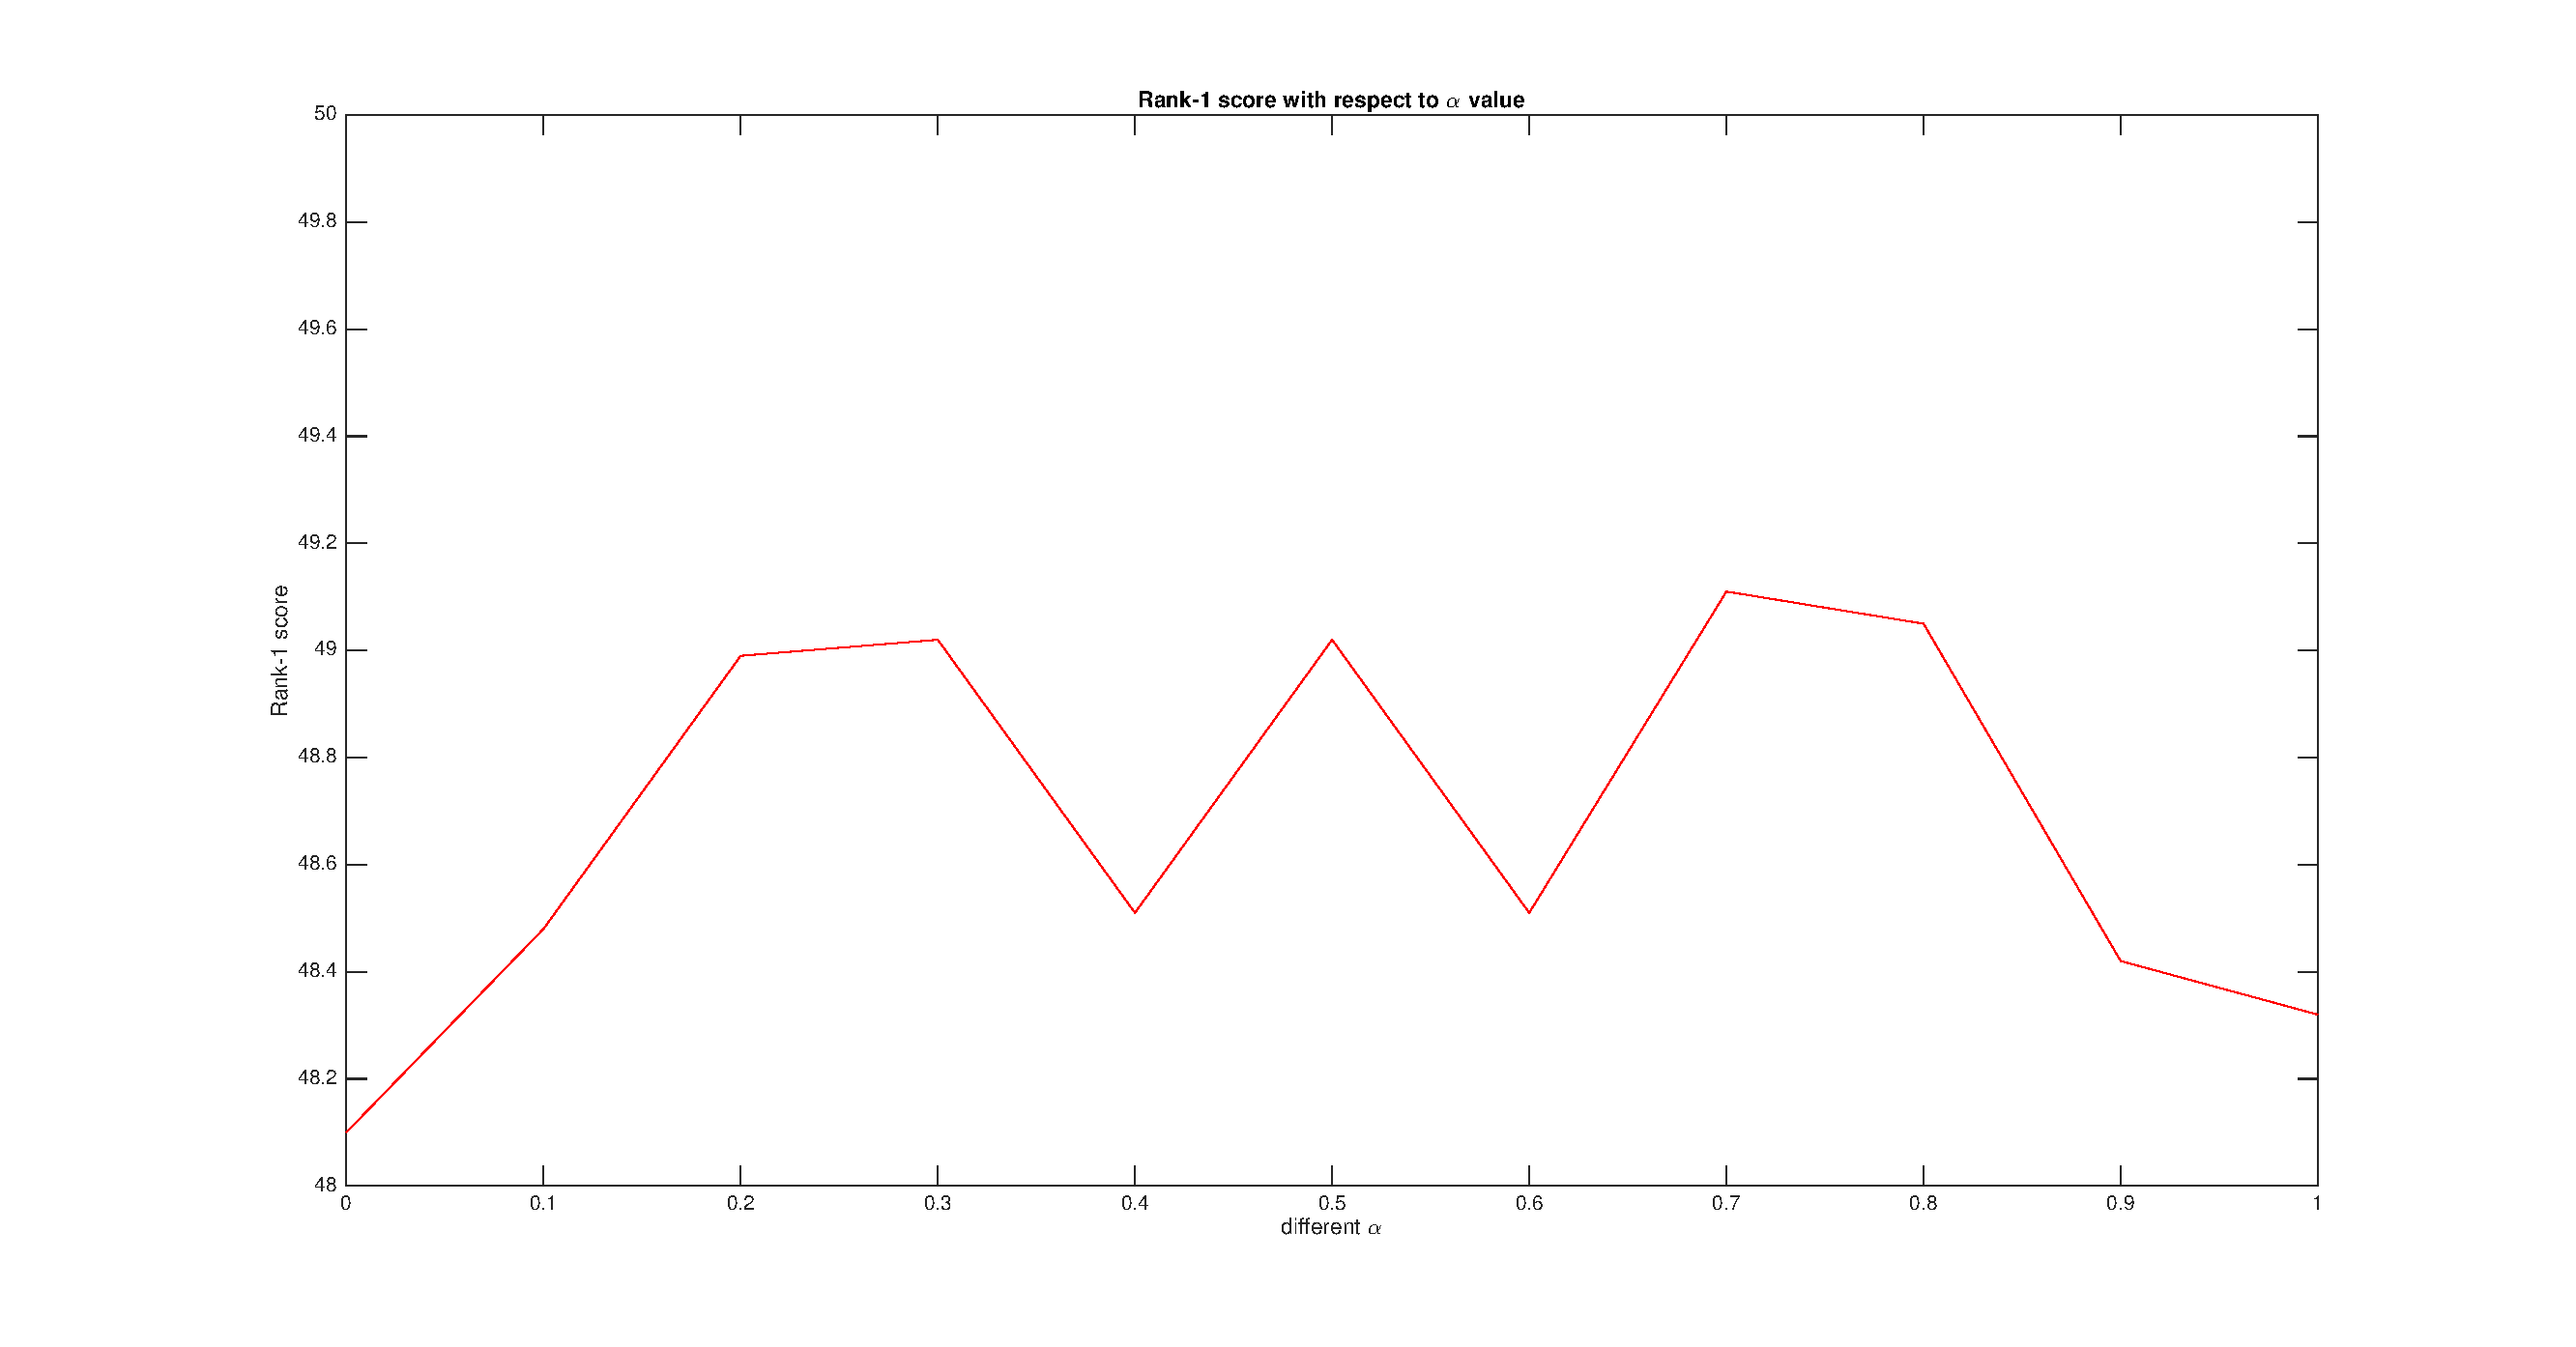
\includegraphics[width=1\linewidth]{/Users/JohnsonJohnson/Downloads/thesis_1/Figures/Rank1scoresAlpha.eps}
\vspace{-3em}
\caption{Rank 1 scores with respect to $\alpha$ on VIPeR}
\end{raggedleft}
\end{figure}
%-------------------------------------------------
\begin{figure}[H]
\begin{raggedleft}
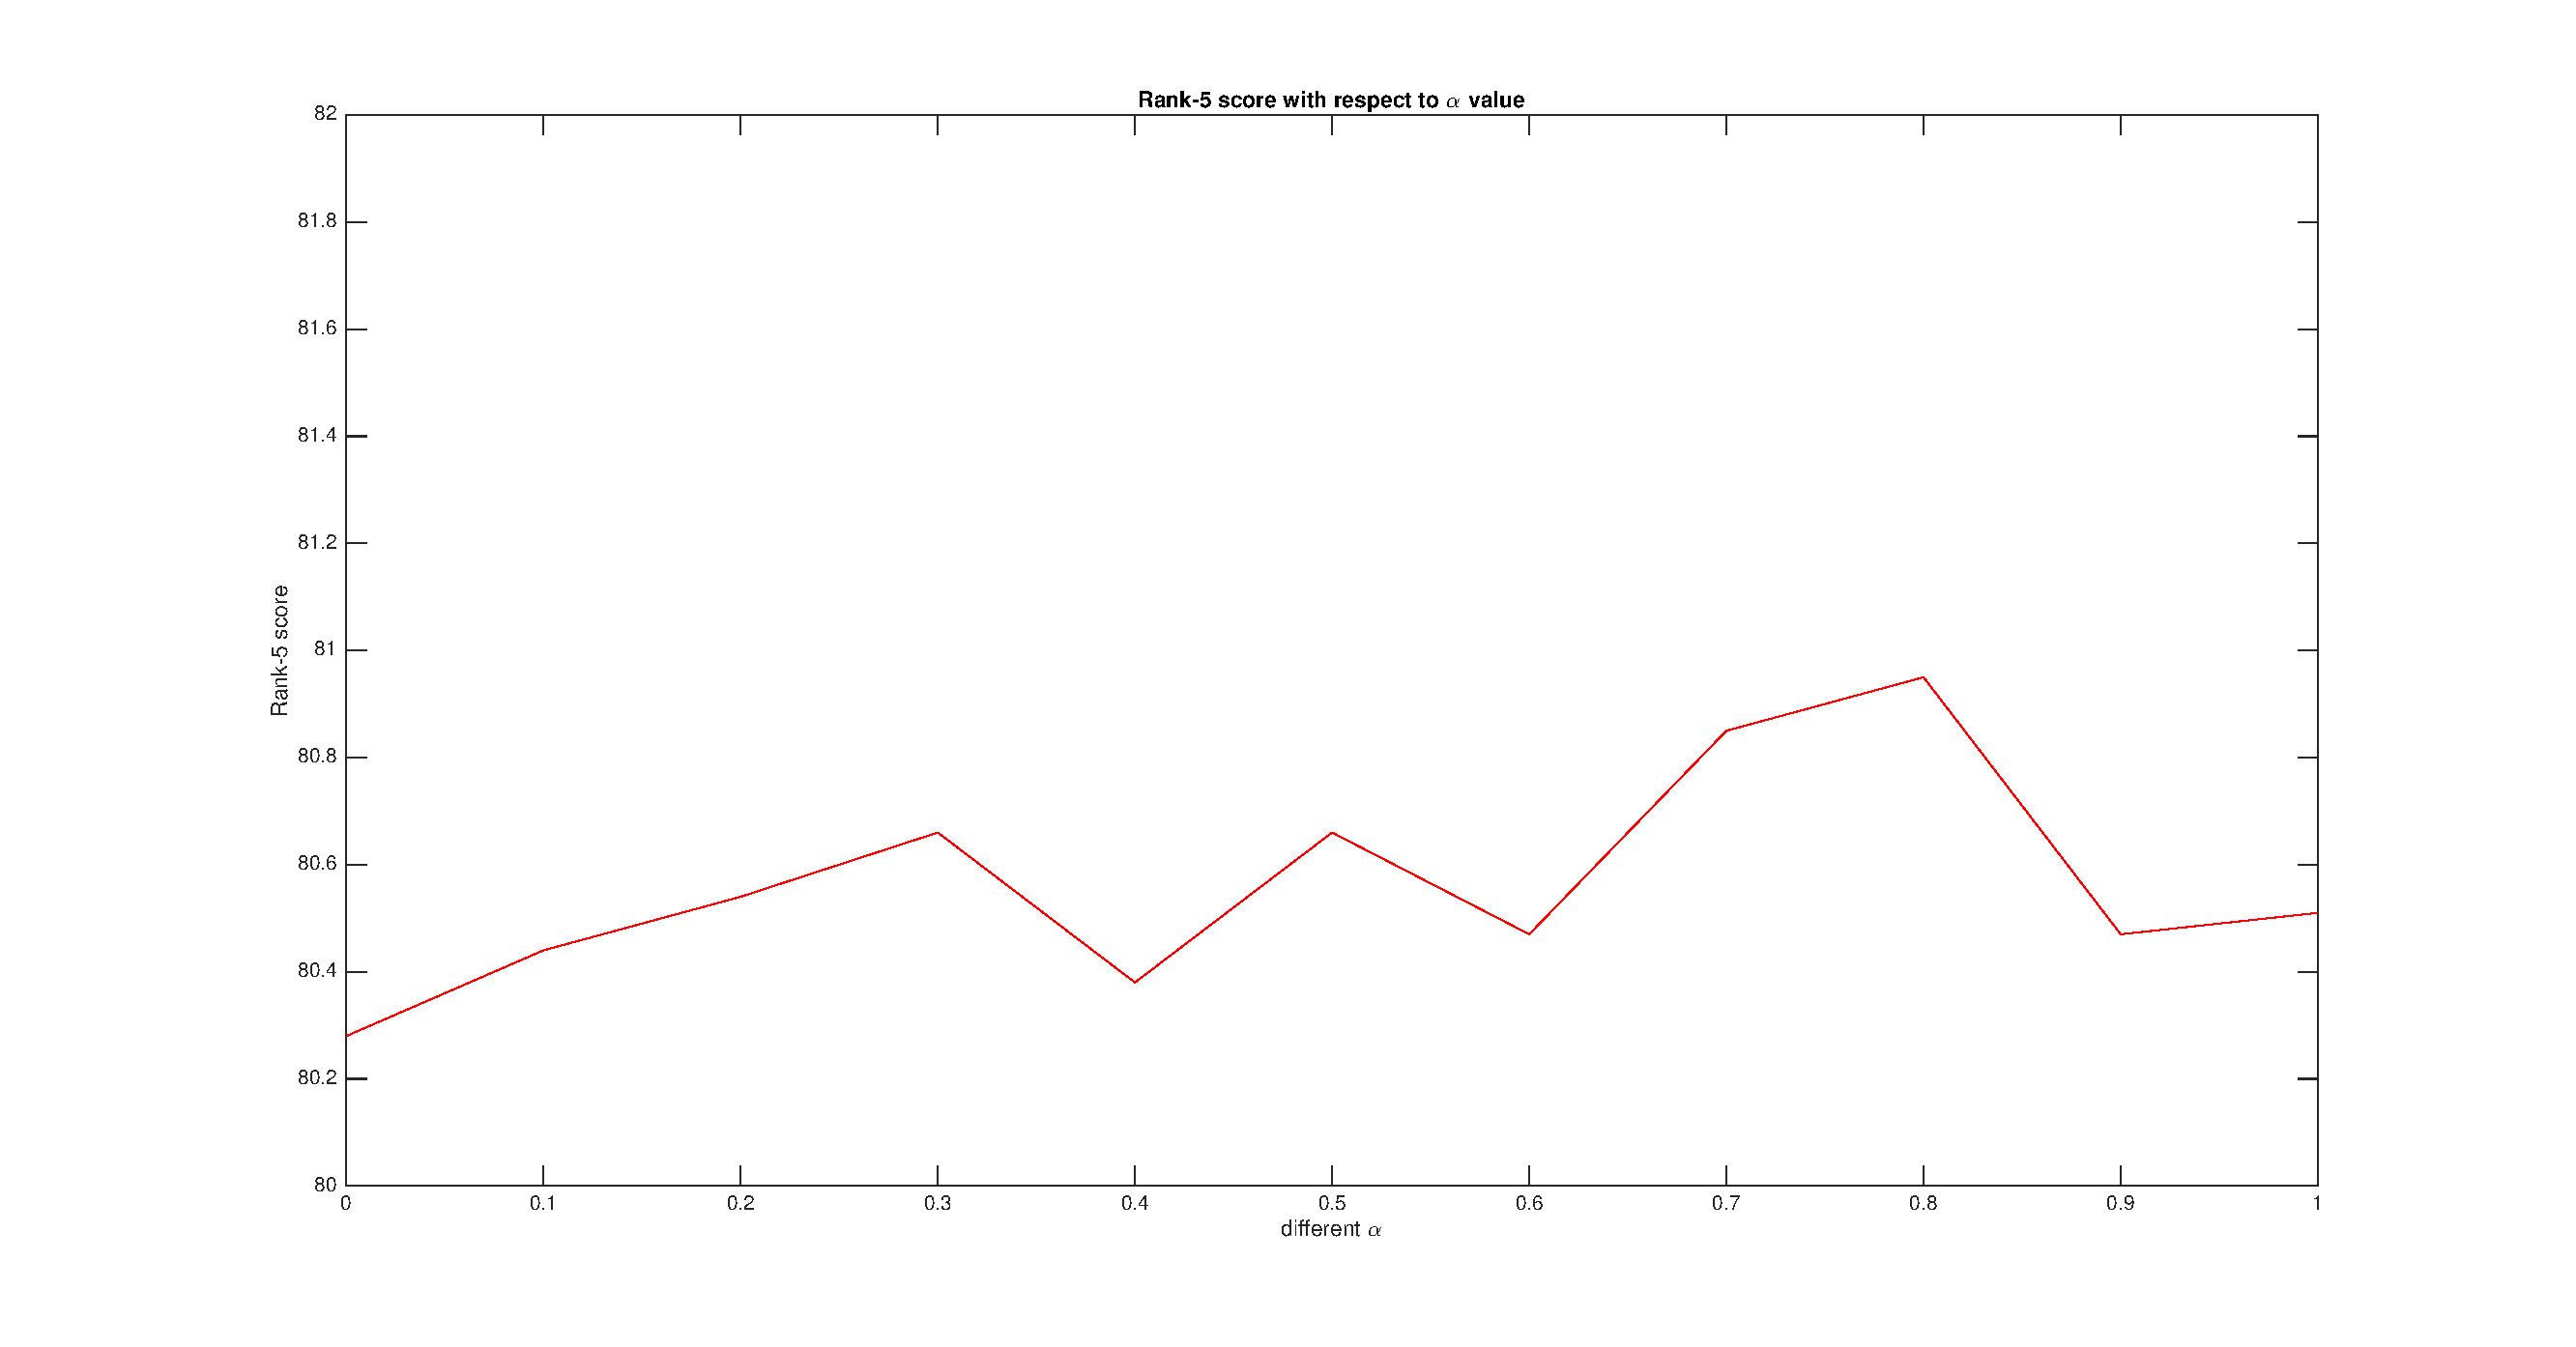
\includegraphics[width=1\linewidth]{/Users/JohnsonJohnson/Downloads/thesis_1/Figures/Rank5scoresAlpha.eps}
\vspace{-3em}
\caption{Rank 5 scores with respect to $\alpha$ on VIPeR}
\end{raggedleft}
\end{figure}
%-------------------------------------------------


\begin{table}[H]
\centering
\caption{Parameters setting}
\begin{tabular}{|l|c|c|c|c|c|}
\hline
Paramters &$\alpha$&thresh&step&Max iteration& slack variable\\
\hline
Values &0.76&$10^{-5}$&0.01&100&1\\
\hline
\end{tabular}
\end{table}


\textbf{Performance measuring} The cumulative matching curve is used to measure the descriptor performance. The score means the probability that the right match is within the top $n$ samples. A perfect CMC curve is expected to have a high rank-1 value and reaches 1 as fast as possible.
%\section{XQDA and NFST}


\section{Performance analysis}
In this paper, we compare proposed metric with other state-of-the-art metrics including NFST[], XQDA[]. NFST is a metric which learn a null space for descriptors so that the the same class descriptors will be projected to  
a single point to minimize within class scatter matrix while different classes are projected to different points. This metric is a good solution to small sample problems in person re-identification. XQDA is quite similar with many other metrics, which learns a projection matrix $W$ and then a Mahanalobis SPD matrix $M$ is learned in the subspace. Those two metric are proved to have state-of-the-art performance with many other methods. The GOGrgb in all forms stands for the hierarchical gaussian descriptor in RGB color space while GOGfusion stands for the one in four different color spaces \{RGB,Lab,HSV,nRnR\}.\\
\textbf{VIPeR} A comparison form is given in Table 8. Some of recent results are also included in this form. We can find that the rank scores are better than those of NFST and XQDA in terms of both GOGrgb and GOGfusion. More specifically, the rank 1, rank 5, rank 10, rank 15 and rank 20 GOGrgb scores of proposed metric learning are 0.44\%, 0.72\%, 1.27\%, 1.3\%, 1.47\% higher than those of GOGrgb+XQDA, and the rank-1, rank-5, rank-10, rank-15 and rank-20 GOGfusion scores of proposed metric learning are 0.19\%, -0.79\%, 0.86\%, 0.63\%, 0.67\% higher than GOGfusion + XQDA respectively. Also we can see that the proposed metric learning has a way more better performance than NFST. We can infer that the performance of KLFDA is better than XQDA, with its rank-1 score 1.6\% higher.  \newline 
%-----------------------------------------------------------------------VIPeR
\begin{table}[H]
\caption{Performance of different metrics on VIPeR}
\centering
 \begin{tabular}{|l|c|c|c|c|c|c|}
\hline
& \multicolumn{5}{|c|}{Rank(\%)} \\
\hline
Methods& 1 & 5 &10& 15&20\\
\hline
GOGrgb+NFST& 43.23&73.16 &83.64 & 89.59&92.88\\  
\hline
GOGrgb+XQDA& 43.01&73.92&83.86& 89.24& 92.37\\
\hline
%GOGrgb+KLFDA&43.45 &74.68 &85.13 &90.54&93.70\\ 
%\hline
GOGrgb+Proposed&43.48&74.59&85.35&90.47&93.67\\   %43.48%, 74.59%, 85.35%, 90.47%, 93.67%
\hline
GOGfusion+NFST&47.15& 76.39&87.31&91.74&94.49\\
\hline
GOGfusion+XQDA& 47.97& 77.44& 86.80& 91.27&93.70\\  
\hline
%GOGfusion+KLFDA & 47.97&77.06& 87.56&91.80&94.18\\
%\hline
GOGfusion+Proposed&48.16& 76.65&87.66&91.90&94.37\\ %48.16%, 76.65%, 87.66%, 91.90%, 94.37%

\hline

%--------------------------------------------------------------
\end{tabular}
\end{table}
\textbf{CUHK1} We can find that the rank 1, rank5, rank 10, rank 15, rank 20 score of GOGrgb combined with proposed metric are 5.35\%, 4.22\%,3.35\%,2.1\%,1.44\% higher than XQDA, and 0.26\%,1.26\%,1.38\%,1.11\%, 1.09\% than NFST.  Also the  rank 1, rank5, rank 10, rank 15, rank 20 score of GOGfusion combined with proposed metric are 4.59\%, 2.55\%, 0.72\%, 1.29\%, 0.89\% higher than GOGfusion combined with XQDA, and 0.4\%, 0.74\%, 0.6\%, 1.05\%, 1.2\% than GOGfusion combined with NFST. 

\begin{figure}[H]
\begin{raggedleft}
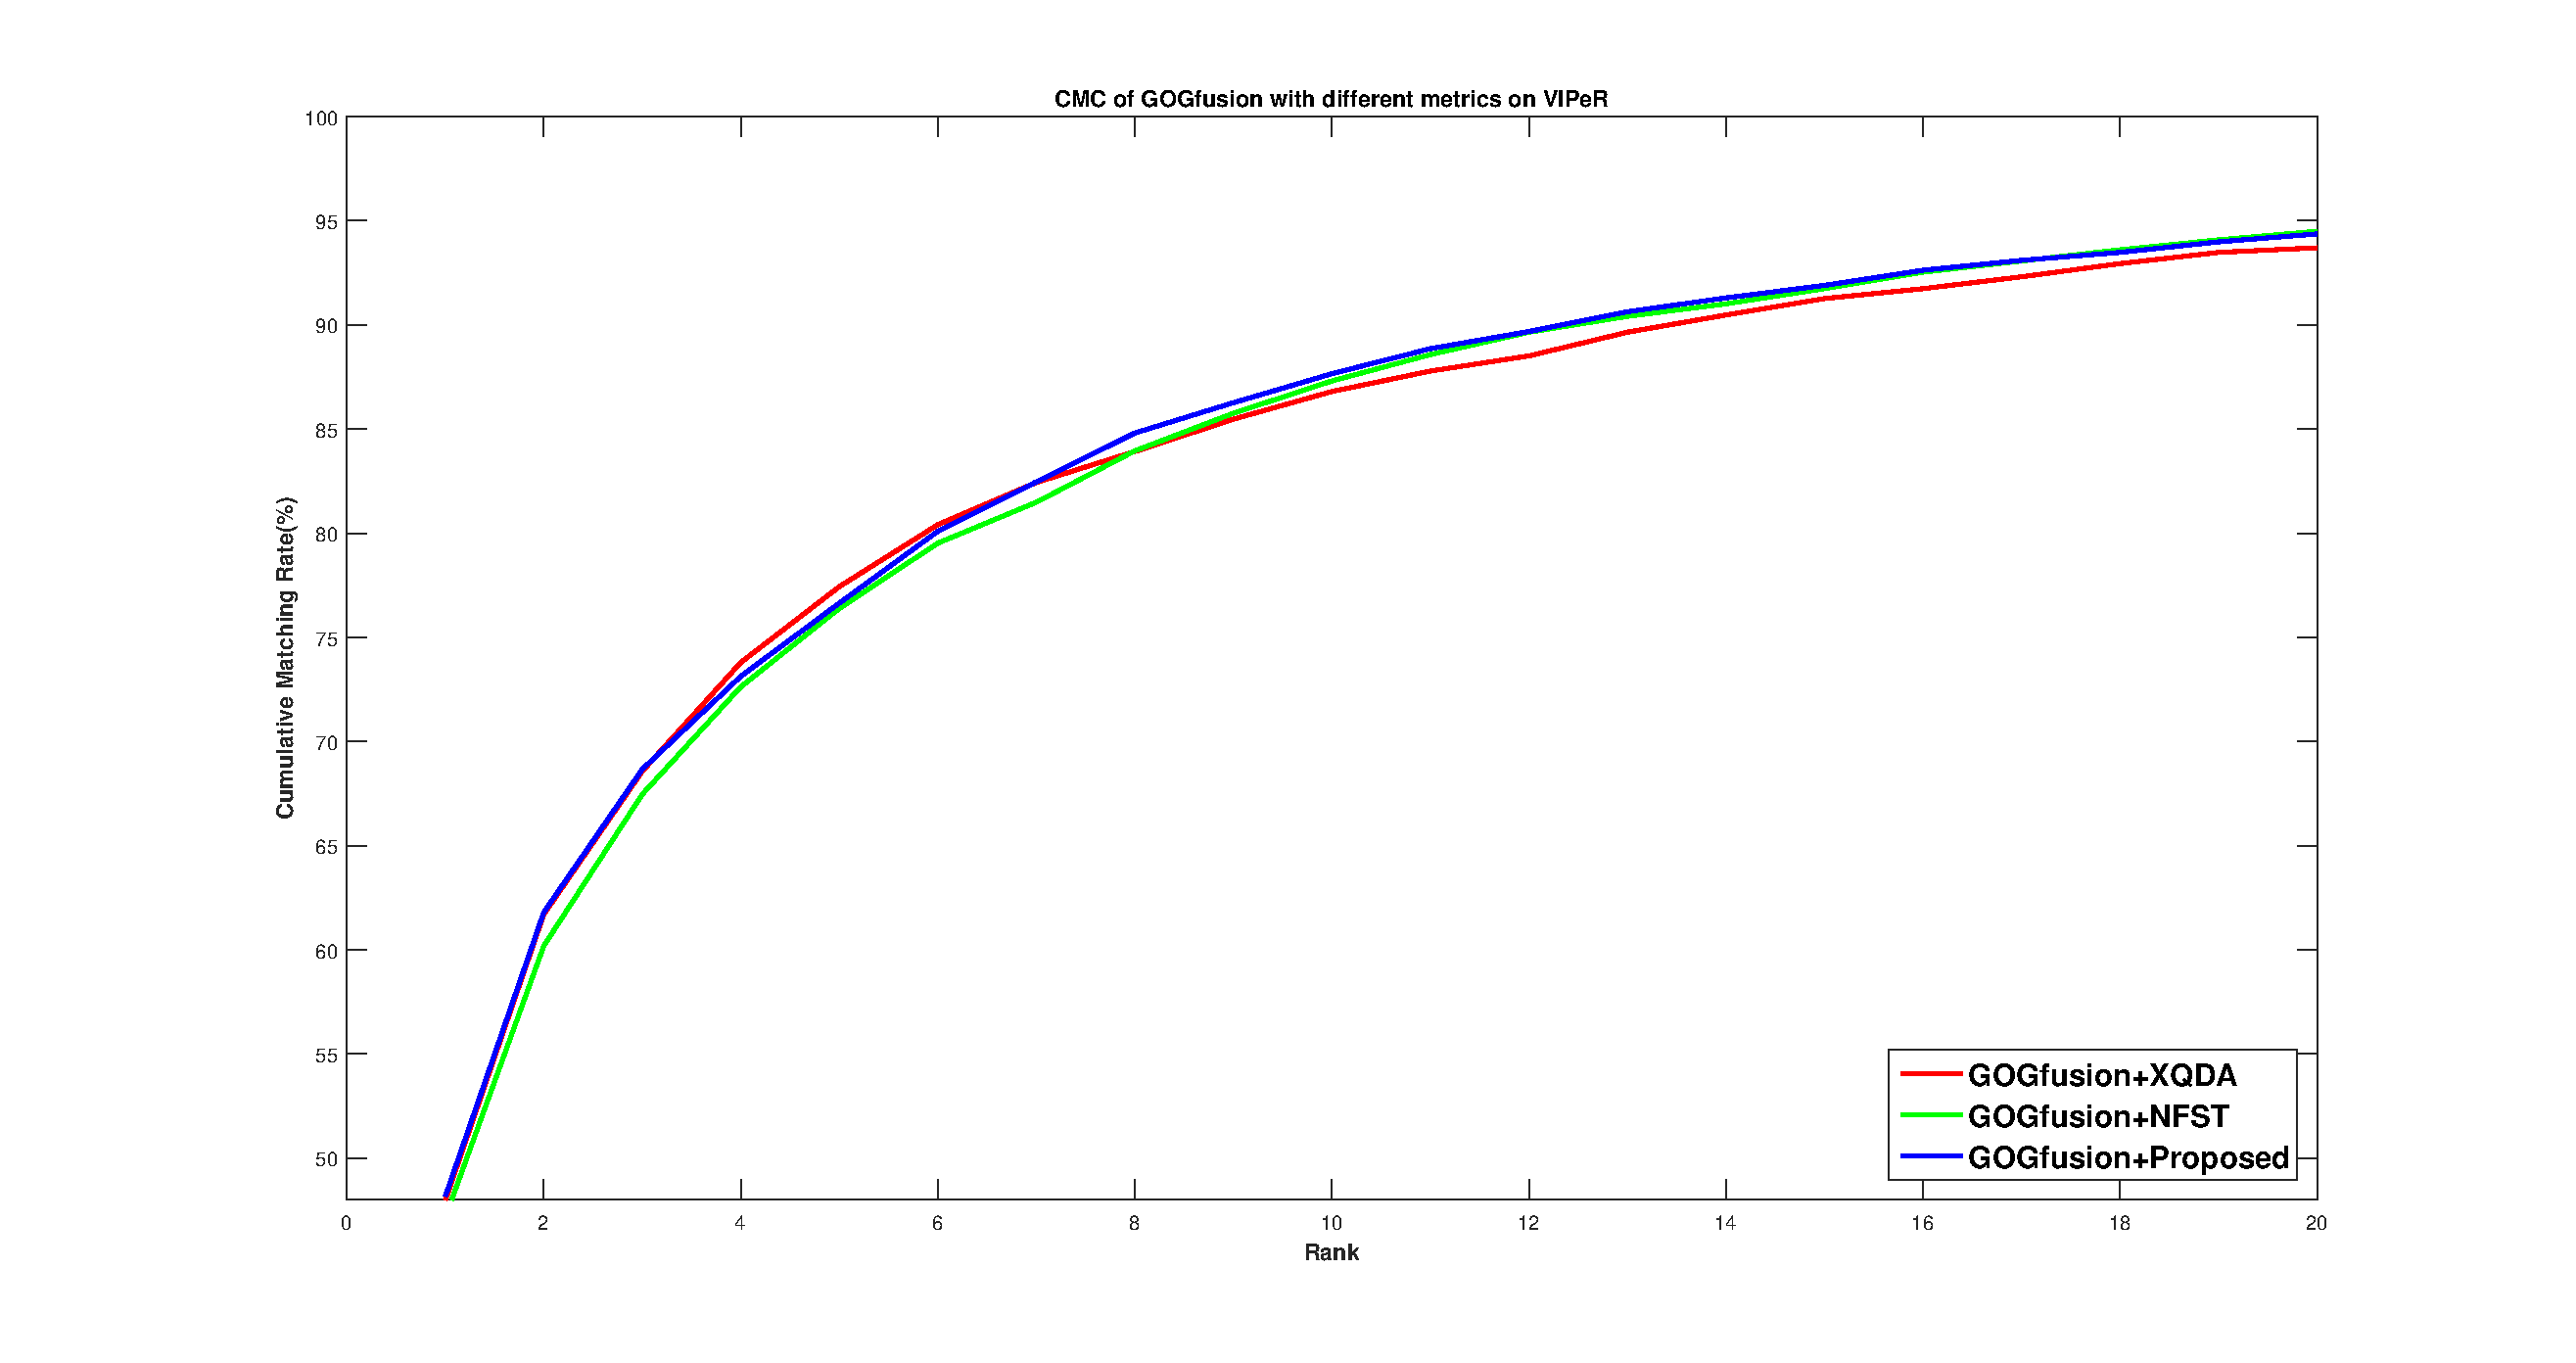
\includegraphics[width=1\linewidth]{/Users/JohnsonJohnson/Downloads/thesis_1/Figures/VIPeR.eps}
\vspace{-3em}
\caption{CMC curves on VIPeR comparing different metric learning}
\end{raggedleft}
\end{figure}
%-------------------------------

%-----------------------------------------------------------------------CUHK1
\begin{table}[H]
\caption{Performance of different metrics on CUHK1}
\centering
\begin{tabular}{|l|c|c|c|c|c|c|}
\hline
& \multicolumn{5}{|c|}{Rank(\%)} \\
\hline
Methods& 1 & 5 &10&15& 20\\
\hline
GOGrgb+NFST&55.60 &83.02 &89.07 &91.98&93.56 \\ 
\hline
GOGrgb+XQDA&50.51 &80.06 &87.10 &90.99&93.21 \\ 
\hline
%GOGrgb+KLFDA&55.66&84.32&90.66&93.07& 94.63\\
%\hline
GOGrgb+Proposed&55.86&84.28&90.45&93.09&94.65\\  %55.86%, 84.28%, 90.45%, 93.09%, 94.65%
\hline
GOGfusion+NFST&56.26 &83.66 &89.63 &92.22&93.70 \\ 
\hline
GOGfusion+XQDA&52.10 &81.85&88.81 &91.98&94.01\\ 
\hline
%GOGfusion+KLFDA & 56.60&84.67&90.41&93.13&94.81\\
%\hline
GOGfusion+Proposed&56.69&84.40&90.53& 93.27&94.90\\

\hline

\end{tabular}\newline
\end{table}
\centering

\begin{figure}[H]
%\begin{raggedleft}
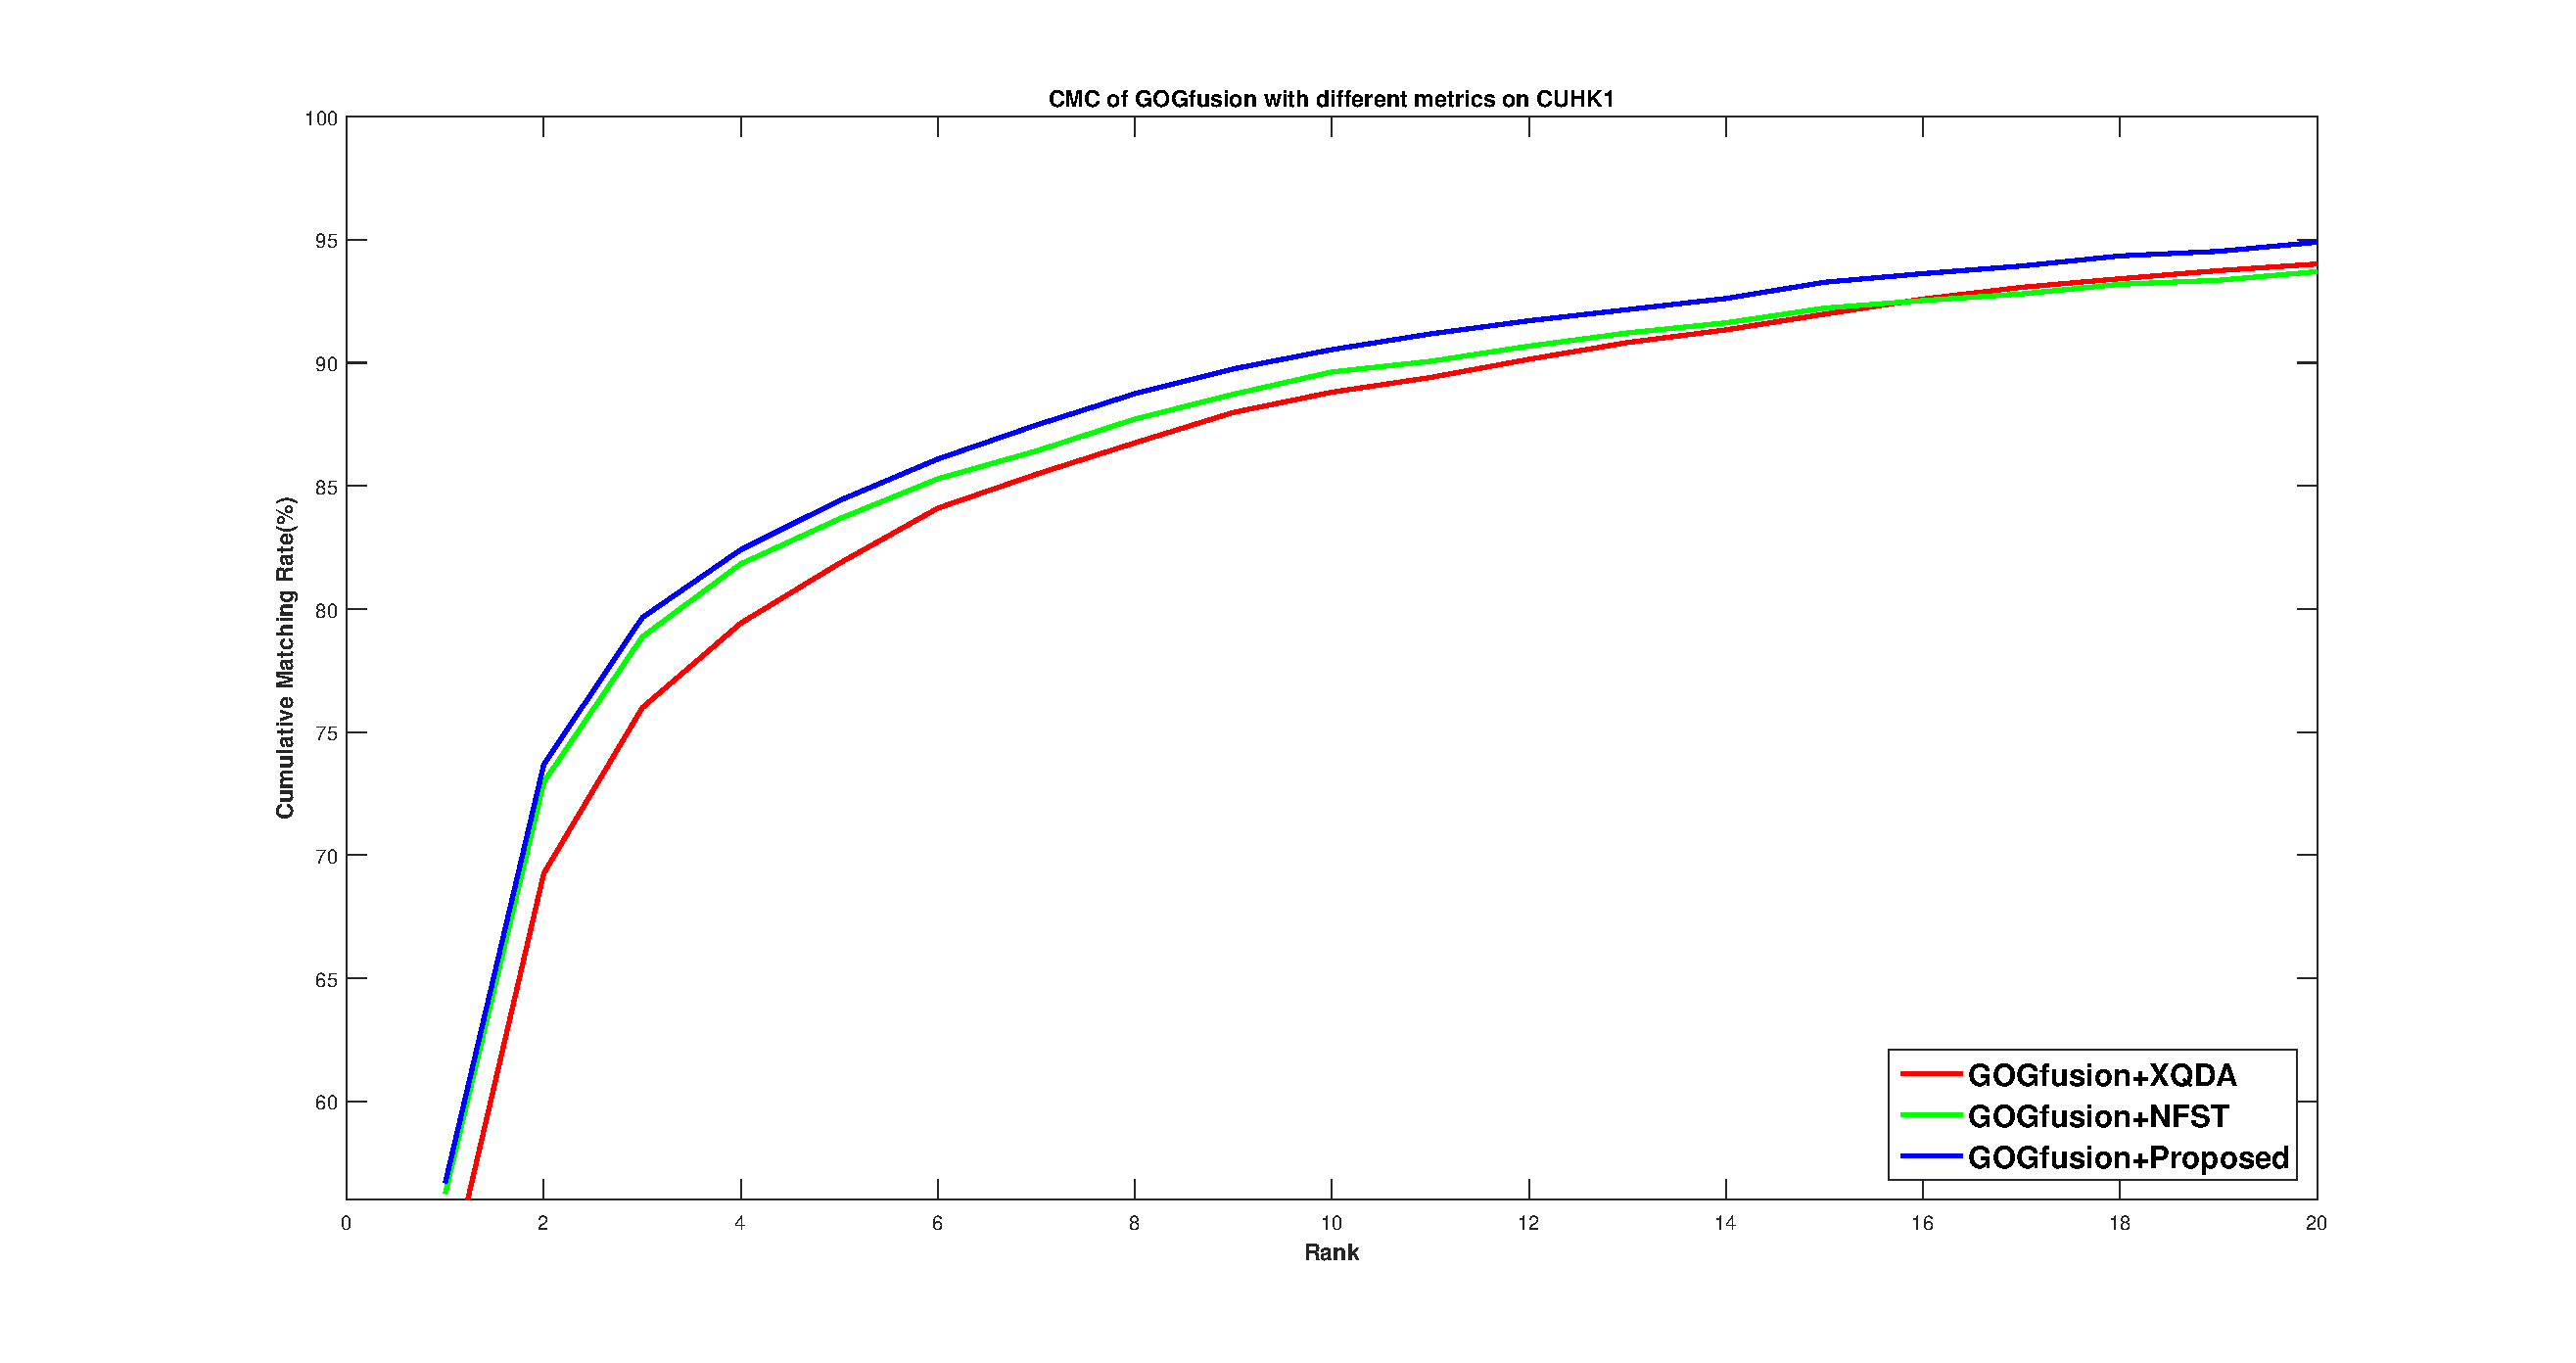
\includegraphics[width=1\linewidth]{/Users/JohnsonJohnson/Downloads/thesis_1/Figures/CUHK1.eps}
\vspace{-3em}
\caption{CMC curves on CUHK1 comparing different metric learning}
%\end{raggedleft}
\end{figure}

%-----------------------------------------------------------------------PRID_2011


\begin{table}[H]
\caption{Performance of different metrics on prid\_2011}
\centering
\begin{tabular}{|l|c|c|c|c|c|c|}
\hline
& \multicolumn{5}{|c|}{Rank(\%)} \\
\hline
Methods& 1 & 5 &10& 15&20\\
\hline
GOGrgb+NFST&26.60 &53.80& 62.90&71.30&75.40 \\ 
\hline
GOGrgb+XQDA&31.10 & 55.70& 66.10 & 72.40&76.10\\  
\hline
%GOGrgb+KLFDA&23.70&51.70&63.10&69.90&73.60\\ 
%\hline
GOGrgb+Proposed&23.80& 52.10& 63.50&70.20&73.50\\  %23.80%, 52.10%, 63.50%, 70.20%, 73.50%
\hline
GOGfusion+NFST&34.10 &58.30& 67.60&73.80&78.30 \\  
\hline
GOGfusion+XQDA&38.40& 61.30&70.80&75.60&79.30\\
\hline
%GOGfusion+KLFDA & 31.90&56.90&66.60&72.60&77.50\\
%\hline
GOGfusion+Proposed&32.20&57.50&66.40&73.50&78.00\\ %32.20%, 57.50%, 66.40%, 73.50%, 78.00%

\hline

\end{tabular}\newline
\end{table}

\textbf{Prid\_2011}  The  rank 1, rank5, rank 10, rank 15, rank 20 score of GOGfusion  combined with proposed metric are 6.2\%, 3.8\%, 4.4\%, 2.1\% and 1.3\% lower than GOGfusion combined with XQDA. The performance of NFST is slightly better than proposed metric. Also in terms of GOGrgb XQDA and NFST has better performance than the proposed one. So in this dataset the proposed metric has worse performance than XQDA and NFST.

\begin{figure}[H]
\begin{raggedleft}
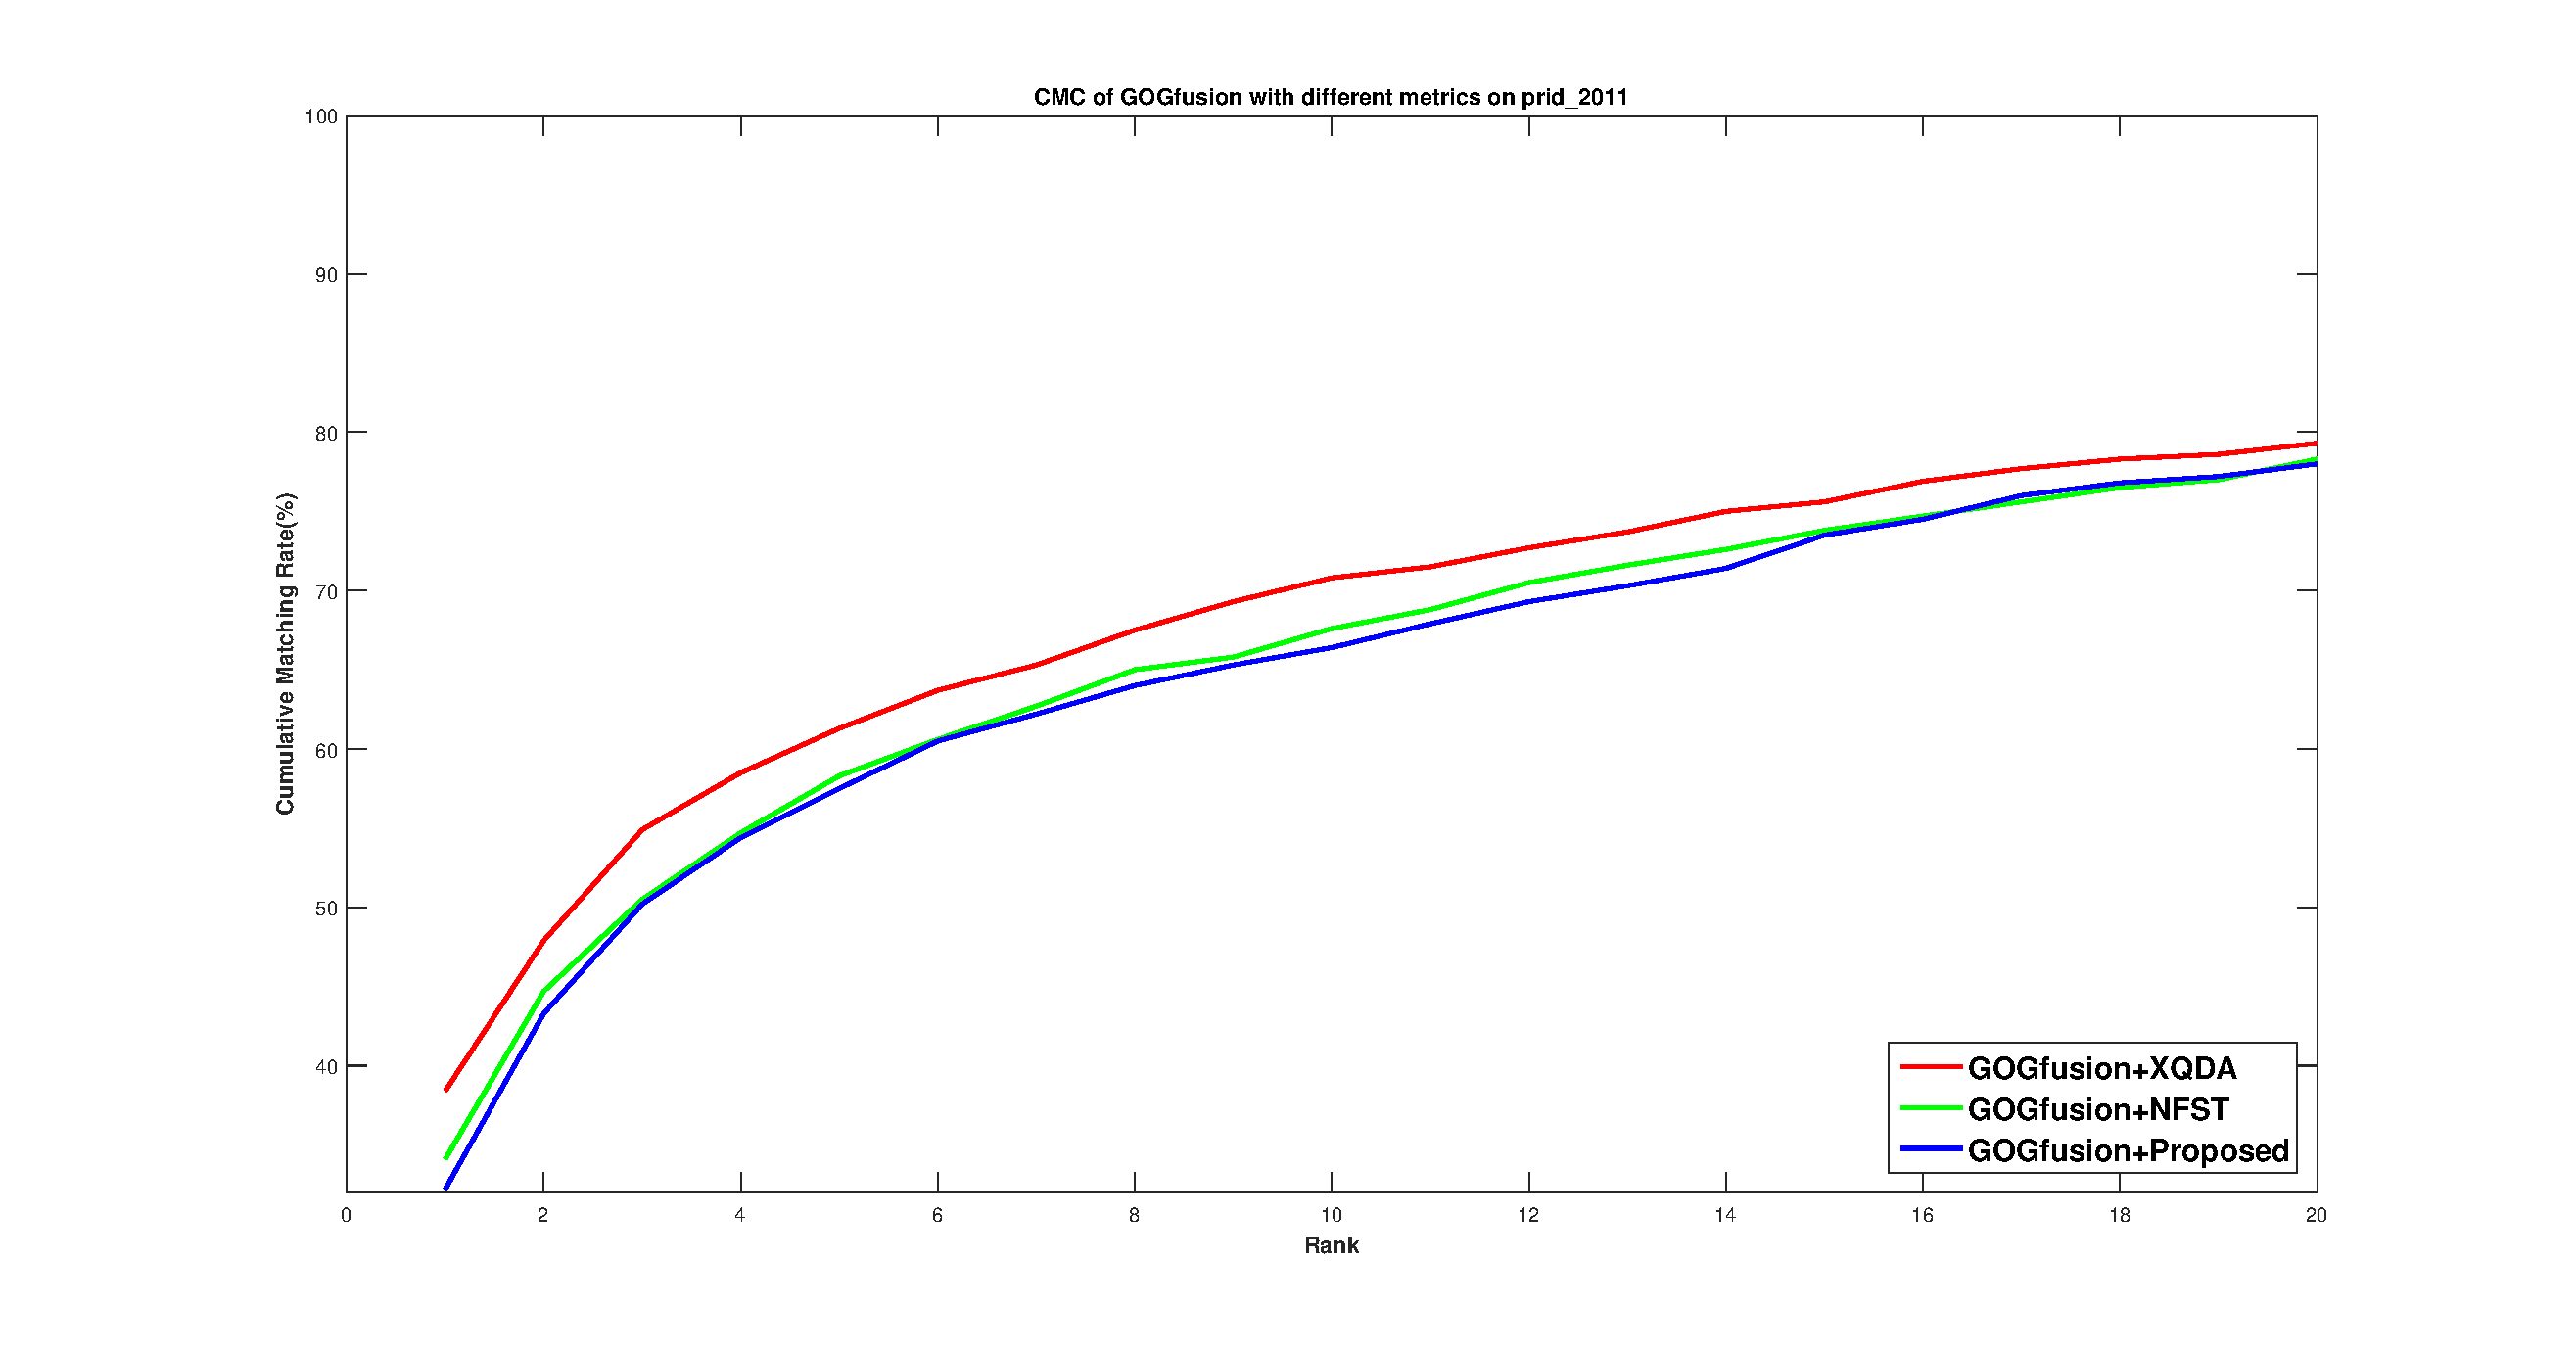
\includegraphics[width=1\linewidth]{/Users/JohnsonJohnson/Downloads/thesis_1/Figures/prid2011.eps}
\vspace{-3em}
\caption{CMC curves on prid\_2011 comparing different metric learning}
\end{raggedleft}
\end{figure}

%-----------------------------------------------------------------------PRID_450S
\begin{table}[H]
\caption{Performance of different metrics on prid\_450s}
\centering
\begin{tabular}{|l|c|c|c|c|c|c|}
\hline
& \multicolumn{5}{|c|}{Rank(\%)} \\
\hline
Methods& 1 & 5 &10& 15&20\\
\hline
GOGrgb+NFST& 61.96&84.98 &90.53& 94.09&96.09 \\  %61.96%, 84.98%, 90.53%, 94.09%, 96.09%
\hline
GOGrgb+XQDA&65.29 &85.02 & 91.13&94.76& 96.49\\ 
\hline
%GOGrgb+KLFDA&60.04&84.09&90.93&94.04&96.00 \\ 
%\hline
GOGrgb+Proposed&60.44& 84.44&91.33&94.00&96.13\\  %60.44%, 84.44%, 91.33%, 94.00%, 96.13%
\hline
GOGfusion+NFST& 64.53&86.62 & 92.93&95.78&97.42 \\ 
\hline
GOGfusion+XQDA&68.40 & 87.42&93.47 &95.69& 97.02\\ 
\hline
%GOGfusion+KLFDA & 62.58&86.18&92.18&95.11&96.84\\
%\hline
GOGfusion+Proposed&62.62&86.44&92.36&95.20& 96.93\\ % 62.62%, 86.44%, 92.36%, 95.20%, 96.93%

\hline

\end{tabular}
\end{table}
\textbf{Prid\_450s} In this dataset, we can find the rank 1 score of XQDA and NFST is higher than proposed metric, but they have almost the same rank 5, rank 10, rank 15, and rank 20 scores with respect to both descriptors. 

\begin{figure}[H]
\begin{raggedleft}
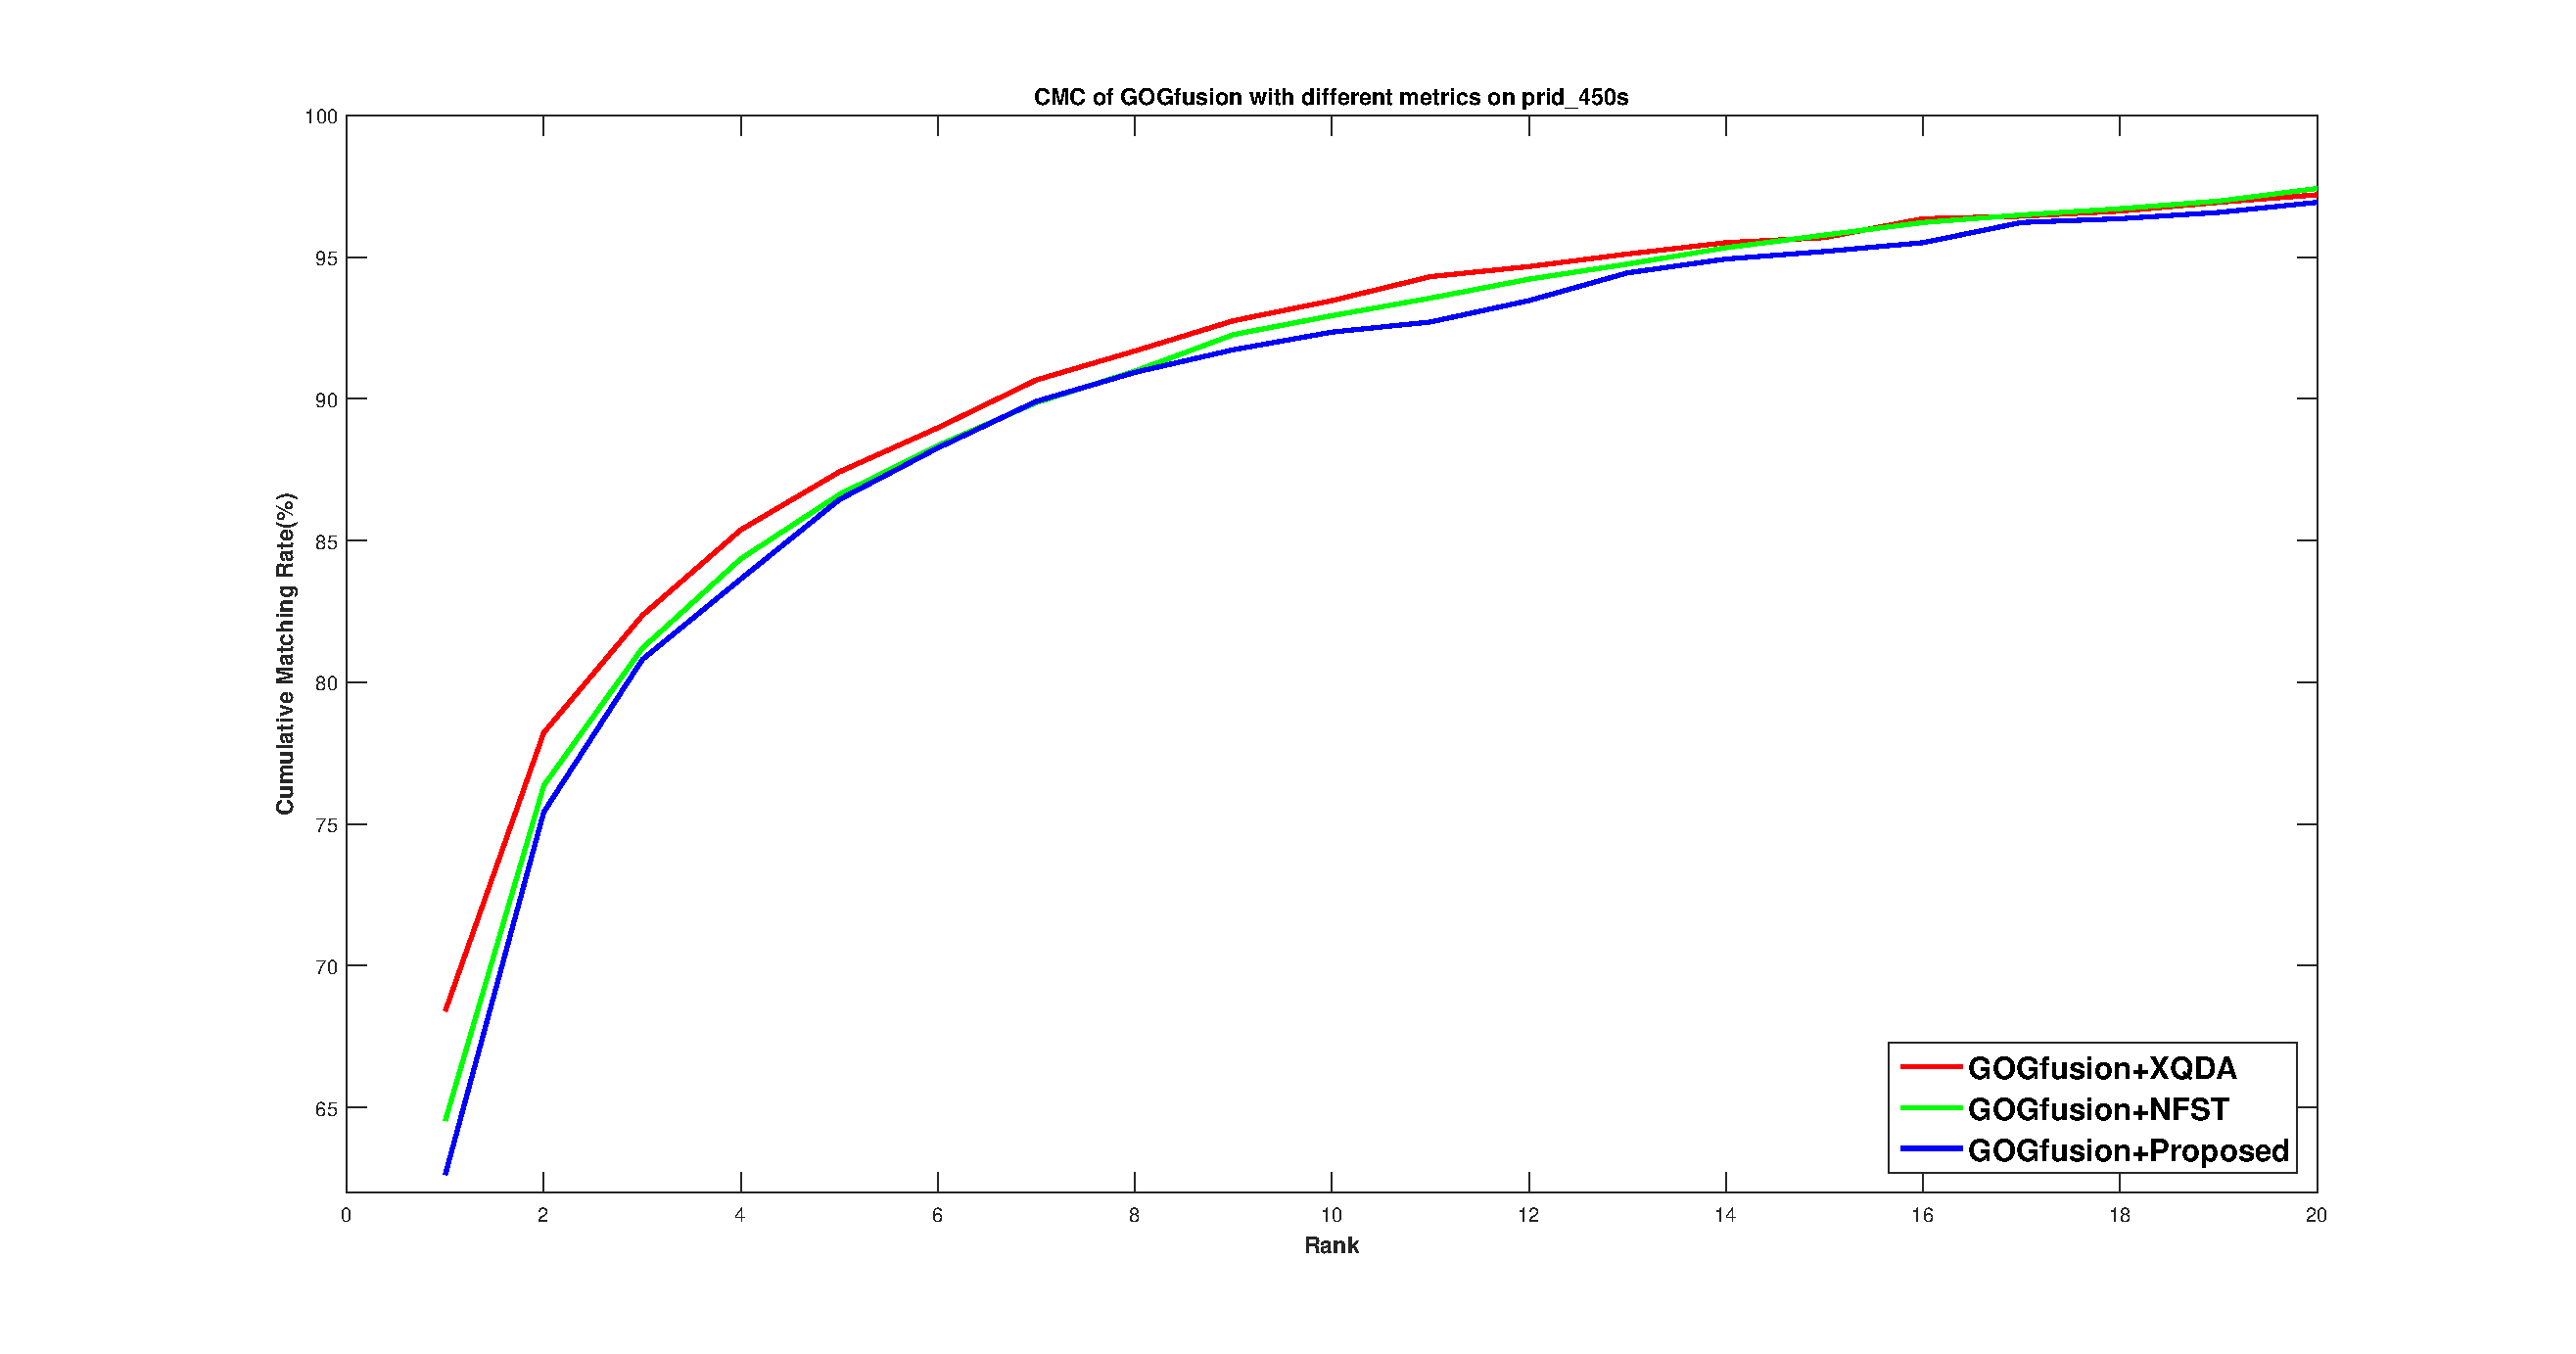
\includegraphics[width=1\linewidth]{/Users/JohnsonJohnson/Downloads/thesis_1/Figures/prid450s.eps}
\vspace{-3em}
\caption{CMC curves on prid\_450s comparing different metric learning}
\end{raggedleft}
\end{figure}

%-----------------------------------------------------------------------GRID
\begin{table}[H]
\caption{Performance of different metrics on GRID}
\centering
\begin{tabular}{|l|c|c|c|c|c|c|}
\hline
& \multicolumn{5}{|c|}{Rank(\%)} \\
\hline
Methods& 1 & 5 &10& 15&20\\
\hline
GOGrgb+NFST& 21.84&41.28 &50.96& 57.44&62.88 \\ 
\hline
GOGrgb+XQDA& 22.64&43.92 &55.12 &61.12&66.56\\ 
\hline
%GOGrgb+KLFDA&23.44&43.04&52.16&59.12&64.88 \\ 
%\hline
GOGrgb+Proposed&22.80&43.76&52.08&59.04&65.12\\  %22.80%, 43.76%, 52.08%, 59.04%, 65.12%
\hline
GOGfusion+NFST& 23.04&44.40 &54.40 &61.84&66.56\\ 
\hline
GOGfusion+XQDA& 23.68&47.28 &58.40 &65.84&69.68 \\ 
\hline
%GOGfusion+KLFDA &23.76&44.40& 55.36&61.76& 66.48\\
%\hline
GOGfusion+Proposed&23.84&44.64&55.04&62.24&66.24\\ %23.84%, 44.64%, 55.04%, 62.24%, 66.24%

\hline

\end{tabular}
\end{table}

\begin{figure}[H]
\begin{raggedleft}
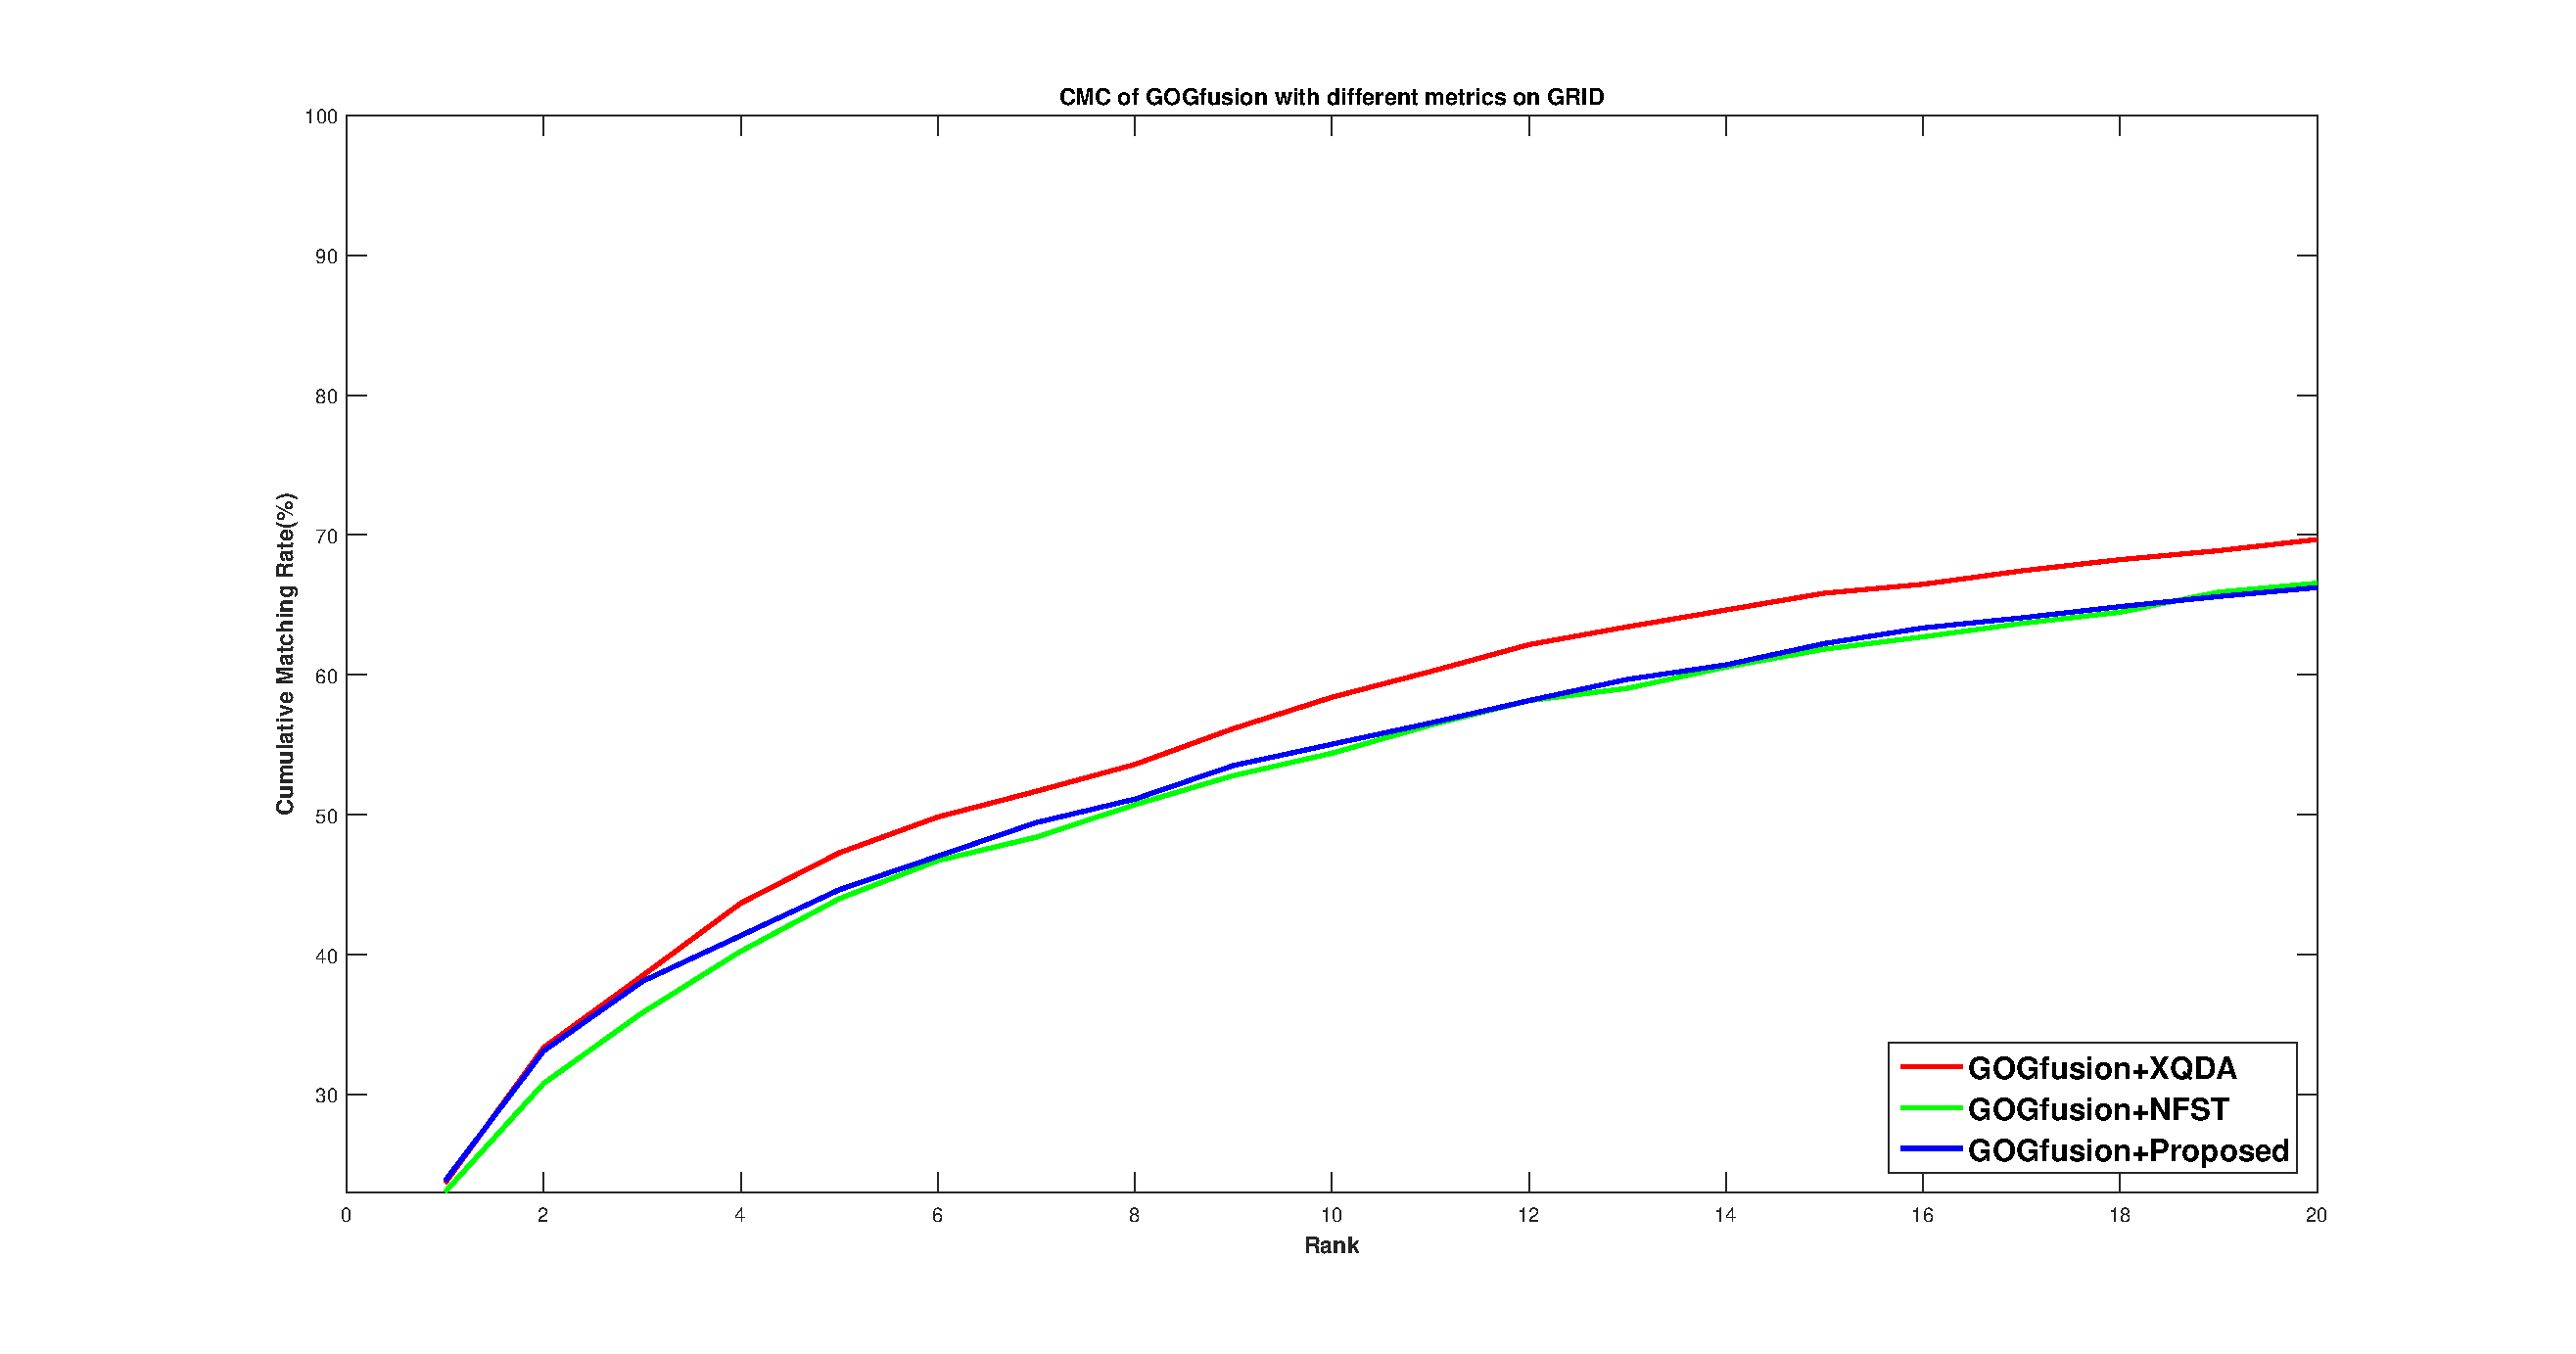
\includegraphics[width=1\linewidth]{/Users/JohnsonJohnson/Downloads/thesis_1/Figures/GRID.eps}
\vspace{-3em}
\caption{CMC curves on GRID comparing different metric learning}
\end{raggedleft}
\end{figure}

\textbf{GRID} We can see that the rank 1 score of proposed metric are slightly higher than XQDA and 0.8\% higher than NFST in terms of GOGfusion, but XQDA outperforms proposed metric on rank 5, rank 10, rank 15 and rank 20 scores. But proposed metric outperforms NFST on rank 5, rank 10, rank 15 and rank 20 scores.
%------------------------------------------------------------------------

